\documentclass{article}
\usepackage[utf8]{inputenc}

\title{}
\date{}

\usepackage[usenames]{color} %used for font color
\usepackage{amssymb} %maths
\usepackage{amsmath} %maths
\usepackage[a4paper, top=3cm, bottom=2.8cm, left=3cm, right=3cm]{geometry}
\usepackage{fancyhdr}
\usepackage[parfill]{parskip}
\setlength{\parindent}{1.5em}
\setlength{\lineskip}{10pt}
\usepackage{indentfirst}
\definecolor{linkblue}{RGB}{50,100,230}
\usepackage[colorlinks=true, linkcolor=linkblue, urlcolor=linkblue, bookmarks=true, linktoc=none]{hyperref}
% \pagestyle{empty}
% \usepackage{booktabs}
\usepackage{graphicx}
\usepackage{tabularx}
\usepackage{multirow}
% \usepackage{polyglossia}
\usepackage{gensymb}
\usepackage{appendix}
\usepackage{mmacells}
\usepackage{minted}
\usepackage{lmodern}
\usepackage{mathtools}
\usepackage{amsthm}
\usepackage{longtable}
\usepackage{titling}
\usepackage[absolute,overlay]{textpos}

\setlength{\TPHorizModule}{1mm}
\setlength{\TPVertModule}{1mm}

\mmaDefineMathReplacement[≤]{<=}{\leq}
\mmaDefineMathReplacement[≥]{>=}{\geq}
\mmaDefineMathReplacement[≠]{!=}{\neq}
\mmaDefineMathReplacement[→]{->}{\to}[2]
\mmaDefineMathReplacement[⧴]{:>}{:\hspace{-.2em}\to}[2]
\mmaDefineMathReplacement{∉}{\notin}
\mmaDefineMathReplacement{∞}{\infty}
\mmaDefineMathReplacement{��}{\mathbbm{d}}

\mmaSet{
  morefv={gobble=2},
  linklocaluri=mma/symbol/definition:#1,
  morecellgraphics={yoffset=1.9ex}
}

\DeclarePairedDelimiter\ceil{\lceil}{\rceil}
\DeclarePairedDelimiter\floor{\lfloor}{\rfloor}

\newcommand\bigfrown[2][\textstyle]{\ensuremath{%
  \array[b]{c}\text{\resizebox{6ex}{.7ex}{$#1\frown$}}\\[-1.3ex]#1#2\endarray}}
  
% \usepackage{times}
\usepackage{newtxtext,newtxmath}

\newtheorem{definition}{Definition}
\newtheorem{theorem}{Theorem}

\pagestyle{fancy}
\lhead{Lecture 1}
\rhead{Handout 1}
\lfoot{Lecture 1}
\rfoot{Handout 1}

\begin{document}
% Initialization commands
\maketitle

\begin{center}
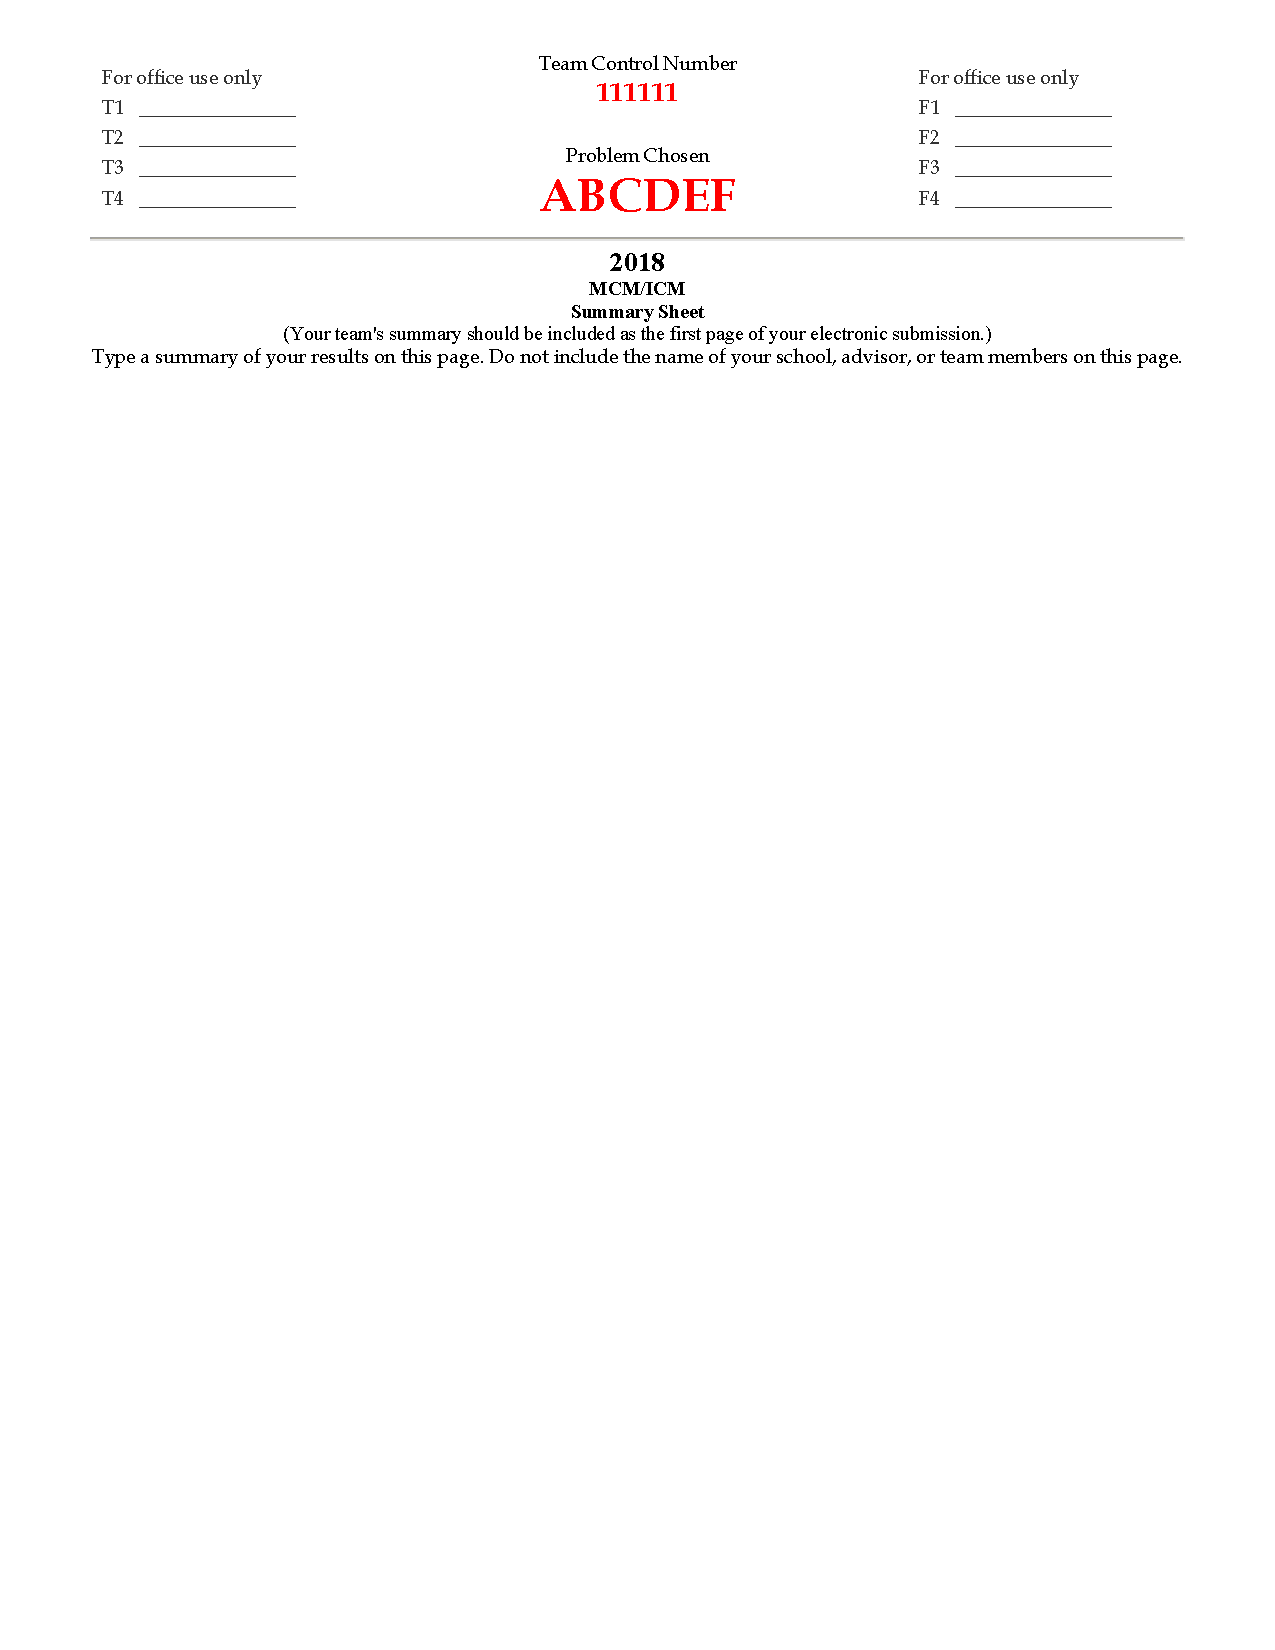
\includegraphics[width=\textwidth, trim=0 600 0 0]{2018Summary.pdf}
\textsc{PROBLEM A \\ Multi-hop HF Radio Propagation}\\[18pt]
\hline\\[8pt]
Team Control Number \\ \textbf{\#81634}
\end{center}

\section*{Summary}

The article extensively uses both univariate and bivariate probability density functions and common proof techniques to approach the ocean reflection problem for both calm and turbulent surfaces. Models that predict the relationships between altitude and multiple attributes of the atmosphere are also developed and presented. Finally, line integral is applied to estimate the expected attenuation of a radio wave that passes the atmosphere at a specific angle.

The article presents an efficient algorithmic method to calculate the reflected vector of any given vector on a spatial surface, and then provides an implementation thereof in Mathematica. The article constructs an polyglot function approximation method, and proves that the Hausdorff distance thereof could be made arbitrarily small.

\pagestyle{fancy}
\fancyhf{}
\rhead{MCM \#81634}
\lhead{Page \thepage}

\newpage
\tableofcontents

\newpage
\section{Introduction}
\subsection{Background}
HF radio wave, electromagnetic wave with frequency interval 3 - 30 mHz, is frequently used in telecommunication in our life. HF radio waves hops inside the earth's atmosphere and attenuate during the process. In order to let all the device to receive the signal, mathematical models need to be created. 
\subsection{Analysis of the Problem}
In this problem, we are required to create models for the propagation of HF radio waves. Three situation are stated in the problem. HF Radio wave & noise in the ocean, HF reflection on land and radio wave receiver on ship. For the first model, we would need to consider th
\section{Assumptions}
Due to the complicated nature of the modeling problem, we introduce several assumptions in order to simplify the construction process of our proposed models.
\begin{enumerate}
    \item \textbf{Water is incompressible.} Water cannot be created nor destroyed, and it's density is uniform in the ocean.
    \item \textbf{The signal reflected by the sea floor is negligible comparing to that by the surface.} Radio wave signal that is transmitted into the water will not exit it again.
    \item \textbf{The surface tension ($\sigma$) of water is constant.}
    \item \textbf{The surface of the ocean is smooth.} The surface (perturbation) of the ocean can be modeled by a continuous function $p(x,y)$ the derivative of which exists up to a sufficient degree at any point in its domain.
    \item \label{apt:tangent} \textbf{The incident radio wave only contacts the ocean surface at an infinitesimal . The region on the ocean surface which scatters the incident radio wave is essentially equivalent to a tangent plane at that point.}
    \item \textbf{The surface of the ocean is clear.} While reflection upon certain objects like boats and leaked oil in the ocean can impact the strength of the reflected signal, we do not take these special circumstances into consideration for sake of simplicity.
    \item \textbf{The change in refractive index across different altitudes in the atmosphere is negligible.} It is assumed electromagnetic waves travel in straight lines between the ionosphere and the surface of the ocean.
    \item \textbf{The surface of the ocean is uniformly continuous.}
    \item \textbf{The density and pressure of the atmosphere can be modeled by probability density functions.}
\end{enumerate}
{\renewcommand{\arraystretch}{1.3}%
\section{Notations}
\begin{center}
    \begin{longtable}{l l{500pt}}
        Notation & Definition \\
        \hline
        $\theta_i$ and $\theta$ & Relative angle of incidence from the ocean surface \\
        $\alpha$ & Absolute angle of incidence from the vertical axis\\
        $Q$ & A point on the ocean surface\\
        $\phi$ & Angular difference between the normal of a point Q and the vertical axis \\
        $\psi$ & Angle of elevation of a radio signal upon entering the ionosphere\\
        $r(\theta_i)$ & A function that returns the reflectance of a calm ocean surface by incident angle\\
        $\sigma$ & Standard deviation of ocean surface normal from the vertical axis\\
        $I$ & Initial strength of a radio wave.\\
        $El$ & Communication Link Elevation\\
        $R_e$ & Effective Earth Radius: 8500km (ITU)\\[20pt]
        \caption{Symbols and definitions.}
    \end{longtable}
    \label{tab:symbol_def}
\end{center}
}


\section{Models}
\subsection{Part I}
\subsubsection{Signal in the Ocean}
\textbf{Part I} of problem A is closely related to multiple laws of wave physics and optics that are relevant to the scattering phenomenon of electromagnetic waves upon a surface. In order to model the behavior of a radio signal wave as it travels from the signal emitter to the signal recipient, several physical facts will be taken for granted and used without proof.

\textbf{\textit{Snell's Law}} establishes a relationship between the angle of incidence \footnote{Angle of incidence} $\theta_i$  and angle of refraction \footnote{Definition} $\theta_r$ when light propagates from one medium to another, when given the \ \footnote{Definition} \textbf{refractive indices} of the two materials. The law is as follows:
\begin{equation}
    n_1 \sin\left(\theta_i\right) = n_2 \sin\left(\theta_r\right)
\end{equation}
where $n_1$ is the refractive index of the first medium and $n_2$ is the refractive index of the second medium.

\textbf{\textit{Fresnel's Equation}} establishes the fraction of the wave that is reflected and the proportion that is transmitted. When an electromagnetic wave propagates from one medium to another with different refractive indices, not 100\% of its energy is reflected back. Part of the energy is transmitted into the second medium. As a result, the overall strength of the signal is reduced. This occurs both when radio wave is incident on the ocean surface and when it propagates through air of non-uniform density. 
When radio waves reflect from the ocean surface, the strength of the reflected wave is determined by the \textbf{reflection coefficient}, or the ratio of the amplitude of the reflected wave to that of the incident wave, $R$. This is the average of the reflectance of the \textbf{p-polarized light}\footnote{The component of the wave that's parallel to the plane of incidence (The plane that contains the incident wave vector.} $R_p$ and the reflectance of the \textbf{s-polarized light}\footnote{The component of the wave that's perpendicular to the plane of incidence} $R_s$.

\begin{equation}
    R_p = \left|\frac{n_1 \cos\theta_r - n_2\cos\theta_i}{n_1\cos\theta_r + n_2 \cos\theta_i}\right|^2 = \left|\frac{n_1 \sqrt{1 - \left(\frac{n_1}{n_2} \sin \theta_i\right)^2} - n_2 \cos \theta_i}{n_1 \sqrt{1 - \left(\frac{n_1}{n_2} \sin \theta_i\right)^2} + n_2 \cos \theta_i}\right|^2
\end{equation}
\begin{equation}
    R_s = \left|\frac{n_1 \cos \theta_i - n_2 \cos \theta_r}{n_1 \cos \theta_i + n_2 \cos \theta_r}\right|^2 = \left|\frac{n_1 \cos \theta_i - n_2 \sqrt{1 - \left(\frac{n_1}{n_2} \sin \theta_i\right)^2}}{n_1 \cos \theta_i + n_2 \sqrt{1 - \left(\frac{n_1}{n_2} \sin \theta_i\right)^2}}\right|^2
\end{equation}
\begin{equation}
    R = \frac{R_p + R_s}{2}
\end{equation}

\subsubsection{First Reflection of Signal from Turbulent Ocean}

The expected reflectance of a turbulent ocean surface differs from that of a calm surface, because when an electromagnetic wave is incident on a particular point $P$ on the water surface whose normal deviates from the vertical $z$ axis, the angle of incidence and angle of reflection will change. Moreover, at particular angles, the reflected wave will be scatter at a direction that again points toward the ocean surface, leading to multiple reflections 

\textbf{\textit{Layers of the Ionosphere}}:

\begin{table}[htbp]
    \centering
    \begin{tabular}{lll}
        Layer name & Range & Reflectivity \\
        \hline
        D Layer & 50-90 km & Low \\
        E Layer & 90-140 km & 10 MHz or lower \\
        F-1 Layer & 150-220 km & High \\
        F-2 Layer & 220-600 km & High
    \end{tabular}
    \caption{Layers of the Ionosphere, Range and Reflectivity}
    \label{tab:ionosphere_levels}
\end{table}

\subsubsection{First Reflection of Signal from Calm Ocean}

The critical difference that lies between the signal strength of a radio wave that reflects from a calm ocean surface and turbulent ocean surface is the proportion of signal that is re-radiated from the surface after the incidence. We need to find a function of incident angle $\theta_i$ that returns the percentage of signal that remains after the first reflection. After research (see appendix), we found that the refractive index of the average ocean surface is at 1.331, and that the average refractive index of Earth's atmosphere at the sea-level is 1.000293. This yields a numeric expression for $r$ in terms of $\theta_i$:
\begin{equation} \label{eqn:r_total}
    r(\theta_i) = \frac{1}{2}\left(\left|\frac{1.000293 \sqrt{1 - \left(0.751 \sin \theta_i\right)^2} - 1.331 \cos \theta_i}{1.000293 \sqrt{1 - \left(0.751 \sin \theta_i\right)^2} + 1.331 \cos \theta_i}\right|^2 + \left|\frac{1.000293 \cos \theta_i - 1.331 \sqrt{1 - \left(0.751 \sin \theta_i\right)^2}}{1.000293 \cos \theta_i + 1.331 \sqrt{1 - \left(0.751 \sin \theta_i\right)^2}}\right|^2\right)
\end{equation}

\begin{figure}[htbp]
    \centering
    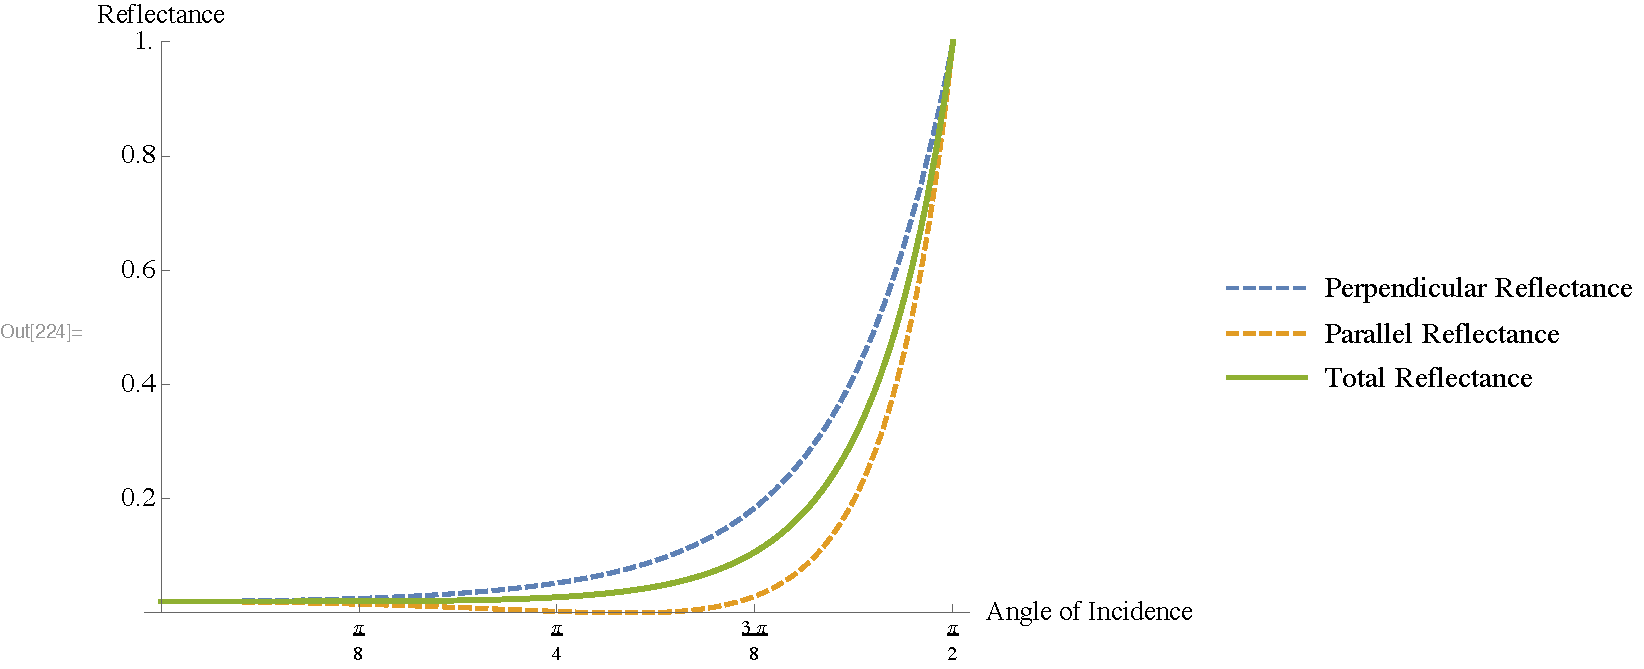
\includegraphics[scale=.55,clip,trim=40 0 6 10]{calm_surface_plot.pdf}
    \caption{Relationship between angle of incidence and reflectance of calm ocean surface.}
    \label{fig:calm_surface_plot}
\end{figure}

When a radio station broadcasts radio signal continuously, it sends radio waves up into the ionosphere, where it is likely to be reflected and sent down to the ground. In the first part, we assume that the signal hits the ocean surface. We may assume the angle which a particular wave is incident at the ocean surface is uniformly distributed from $0$ to $\frac{\pi}{2}$ radians from the normal, with a constant density of $\frac{1}{2\pi}.$ Therefore, figure \ref{fig:calm_surface_plot} can be viewed as a probability density function $r(\theta)$ as shown in equation \eqref{eqn:r_total} for the reflectance of radio waves at calm sea from different angles of incidence. The expected reflectance is \begin{equation}
    \int_0^\frac{\pi}{2} \theta r(\theta) d\theta = 0.2459.
\end{equation}

\subsubsection{First Reflection off a Turbulent Ocean}

The case of a turbulent ocean surface is slightly less straightforward than that of a calm ocean surface, because it is likely that an incident wave will be reflected from a point $P$ on the ocean surface whose normal line is not co-linear with the vertical $z$ axis. Let $\phi_x$ be the $x$-component of the angular difference between the normal line at $P$ and the vertical line, and let $\phi_y$ be the $y$-component of the angular difference. We define the angle of deviation such that if the normal of a facet is to the left of the vertical, then it is negative. Otherwise, it is positive. For a calm surface, $\phi_x$ and $\phi_y$ are uniformly 0.

Consider a $x$-$z$ plane cross-section of a turbulent ocean as shown in figure \ref{fig:line_approx}. It can be shown that the curve of the ocean in this cross-section can be well approximated by connected segments (facets) that intersect $S$.

\phantom{ }
% Using epsilon and delta
\begin{definition}[Uniform Continuity]
A function $f(x)\in C^0(I)$ is consistently continuous if and only if
\[
\forall\varepsilon>0.\,\,\exists\delta>0.\,\,\forall x_1,x_2\in I.\,\,\left|x_1-x_2\right|<\delta\implies\left|f(x_1)-f(x_2)\right|<\varepsilon
\]
\end{definition}

\begin{definition}[$F_\varepsilon$-approximation]
For any function $f(x)$ that is uniformly continuous over a real interval $(m,n)$, $\forall\varepsilon>0$, according to the uniform continuity thereof, $\exists\delta_0>0$ such that $\forall x_1,x_2\in(m,n)$, whenever $\left|x_1-x_2\right|<\delta_0$, $\displaystyle{\left|f(x_1)-f(x_2)\right|<\frac{\varepsilon}{2}}$. Denote $\displaystyle{\delta=\min\left\{\delta_0,\frac{n-m}{2}\right\}}$, and name $\displaystyle{a=m+\frac{\delta}{2},\,\,b=n-\frac{\delta}{2}}$, then divide the interval $[a,b]$ into $\displaystyle{s=\left(\floor*{\frac{b-a}{\delta}}+1\right)}$ partitions, and denote the length of each $L$, and it is obvious that $L<\delta$. Define a sequence $\left\{a_k\right\}$ such that $a_k=a+(k-1)L$, for $k=1,2,\dots,s+1$, thus $a_1=a,\,\,a_{s+1}=b$. Now define the $F_\varepsilon$-approximation function of the uniformly continuous function $f(x)$ as
\begin{align*}
F_\varepsilon(x)=
\begin{cases}
f(a)&m<x<a_1\\
\displaystyle{\frac{f(a_{k+1})-f(a_k)}{a_{k+1}-a_k}}\cdot(x-a_k)+f(a_k)&a_k\leq x<a_{k+1},\,\,k=1,2,\dots,s\\
f(b)&a_{s+1}\leq x<b
\end{cases}
\end{align*}
\end{definition}

\begin{definition}[Functional Distance]
\label{def:functional_distance}
For any $f(x), g(x)$ the domains of which both contain a common open interval $(m,n)$, the distance between these two functions are defined as
\[
d_{(m,n)}(f,g)=\sup_{x\in(m,n)}\left\{\left|f(x)-g(x)\right|\right\}
\]
\end{definition}

\begin{theorem}[Functional Metric]
The functional defined in \ref{def:functional_distance} is a metric of $(m,n)\to\mathbb{R}$.
\end{theorem}
\begin{proof}
Trivial.
\end{proof}

\begin{theorem}[$F_\varepsilon$ Uniform Continuity]
For any function $f(x):(m.n)\to\mathbb{R}$, its $F_\varepsilon$-approximation function is also uniformly continuous over the same domain.
\end{theorem}
\begin{proof}
Trivial.
\end{proof}

\begin{theorem}[$F_\varepsilon$ Distance]
For any function $f(x):(m.n)\to\mathbb{R}$,
\[
d_{(m,n)}(F_\varepsilon,f)<\varepsilon
\]
\end{theorem}
\begin{proof}
Case analysis on $x\in(m,n)$,
\begin{itemize}
\item
$x\in(m,a)$\\
\[
\left|F_\varepsilon(x)-f(x)\right|=\left|f(a)-f(x)\right|<\frac{\varepsilon}{2}
\]
\item
$x\in[a_k,a_{k+1}),\,\,k=1,2,\dots,s$
\begin{align*}
\left|F_\varepsilon(x)-f(x)\right|&=\left|\frac{f(a_{k+1})-f(a_k)}{a_{k+1}-a_k}\cdot(x-a_k)+f(a_k)-f(x)\right|\\
&\leq\left|\frac{f(a_{k+1})-f(a_k)}{a_{k+1}-a_k}\cdot(x-a_k)\right|+\left|f(a_k)-f(x)\right|\\
&<%%%%%%%%%%%%%%%%%%%%% 0\leq(x-a_k)<(a_{k+1}-a_k), x\in[a_k,a_{k+1})
\left|f\left(a_{k+1}\right)-f\left(a_k\right)\right|+\left|f\left(a_k\right)-f\left(x\right)\right|\\
&<\frac{\varepsilon}{2}+\frac{\varepsilon}{2}=\varepsilon
\end{align*}
\item
$x\in[b,n)$\\
\[
\left|F_\varepsilon(x)-f(x)\right|=\left|f(b)-f(x)\right|<\frac{\varepsilon}{2}
\]
\end{itemize}
Thus
\[
d_{(m,n)}(F_\varepsilon,f)=\sup_{x\in(m,n)}\left\{\left|F_\epsilon(x)-f(x)\right|\right\}<\max\left\{\frac{\varepsilon}{2},\varepsilon\right\}=\varepsilon %epsilon>0,最小上界小于epsilon,需要证明,lim epsilon->0 则 d(Fe,f) -> epsilon,其他情况严格小于,因为 epsilon -> 0时,\left(\floor*{\frac{b-a}{\delta}}+1\right) -> epsilon/2, /\, x -> a_k时,f(ak) - f(x) -> epsilon/2, d(Fe,f) -> epsilon,其他情况严格。
\]

Quod erat demonstrandum.
\end{proof}

\begin{figure}[htbp]
   . \centering
    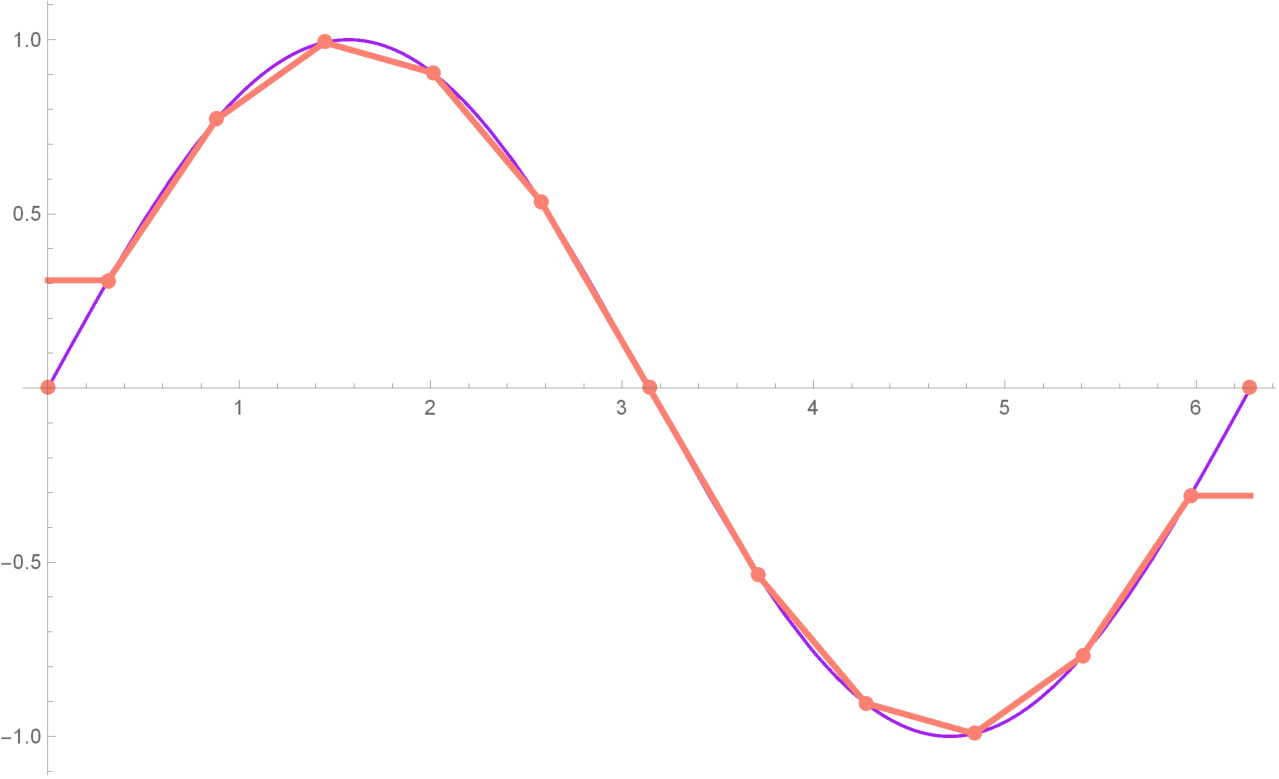
\includegraphics[scale=.6]{approx.pdf}
    \caption{Approximation of turbulent ocean surface by small facets.}
    \label{fig:line_approx}
\end{figure}

Let $\phi_{xi}$ denote the angle of deviation of the $i$-th segment within a given interval. It can be assumed that $\{\phi_{xi}: 1 \le i \le M\}$ follows a normal distribution with mean 0 and unknown standard deviation $\sigma_x$.

\begin{equation}
    \phi_{xi} \sim N(0,\sigma) = \frac{1}{\sigma \sqrt{2\pi}}e^{\frac{-1}{2}\left(\frac{x}{\sigma}\right)^2}
\end{equation}

Similarly, the $y$-component of $\phi$ can be expressed using a the same normal distribution function (i.e. same standard deviation and same mean) with standard deviation $\sigma_y$.

Combining the two variables, we can construct a bivariate normal probability density distribution for random variables $\phi_x$ and $\phi_y$:
\begin{equation}\label{eqn:prob}
    P(\phi_x,\phi_y) = \frac{1}{2\pi \sigma_x \sigma_y \sqrt{1 - \rho^2}} \exp\left[-\frac{1}{2(1-\rho^2)}\left(\frac{\phi_x^2}{\sigma_x^2} + \frac{2\rho \phi_x \phi_y}{\sigma_x \sigma_y} + \frac{\phi_y^2}{\sigma_y^2}\right)\right]
\end{equation}

where $\rho \in (-1,1)$ is the correlation of $\phi_x$ and $\phi_y$, and is defined as:
\begin{equation}
\rho \equiv \mathrm{cor}(\phi_x,\phi_y) \equiv \frac{\mathrm{cov}(\phi_x,\phi_y)}{\sigma_x \sigma_y} \equiv \frac{\mathrm{E}\left(\phi_x \phi_y\right)}{\sqrt{\mathrm{E}\left(\phi_x^2\right)} \sqrt{\mathrm{E}\left(\phi_y^2\right)}}
\end{equation}.

From data provided by NASA on a certain region of the ocean, we computed $\sigma_x$ and $\sigma_y$ as $6.560 \times 10^{-5}$ and $2.916 \times 10^{-5}$ respectively. For details, please see Appendix \ref{sd}.

Note that the \textbf{absolute angle of incidence} $\alpha$ (angle with the vertical axis $z$) does not affect the distribution of the normal on the ocean surface. This is because the normal of a surface is the same for all angles of incidence. Let $\theta$ be the \textbf{relative angle of incidence} (angle relative to the part of the surface which the wave is reflected). Therefore, equation \eqref{eqn:prob} represents a PDF for the distribution of normal for all angles of the incoming wave $\alpha$. Angles $\alpha$, $\theta$ and $\phi$ are also related in the following way:

\begin{align}
    \alpha_x = \theta_x + \phi_x\\
    \alpha_y = \theta_y + \phi_y
\end{align}

\begin{figure}[htbp]
    \centering
    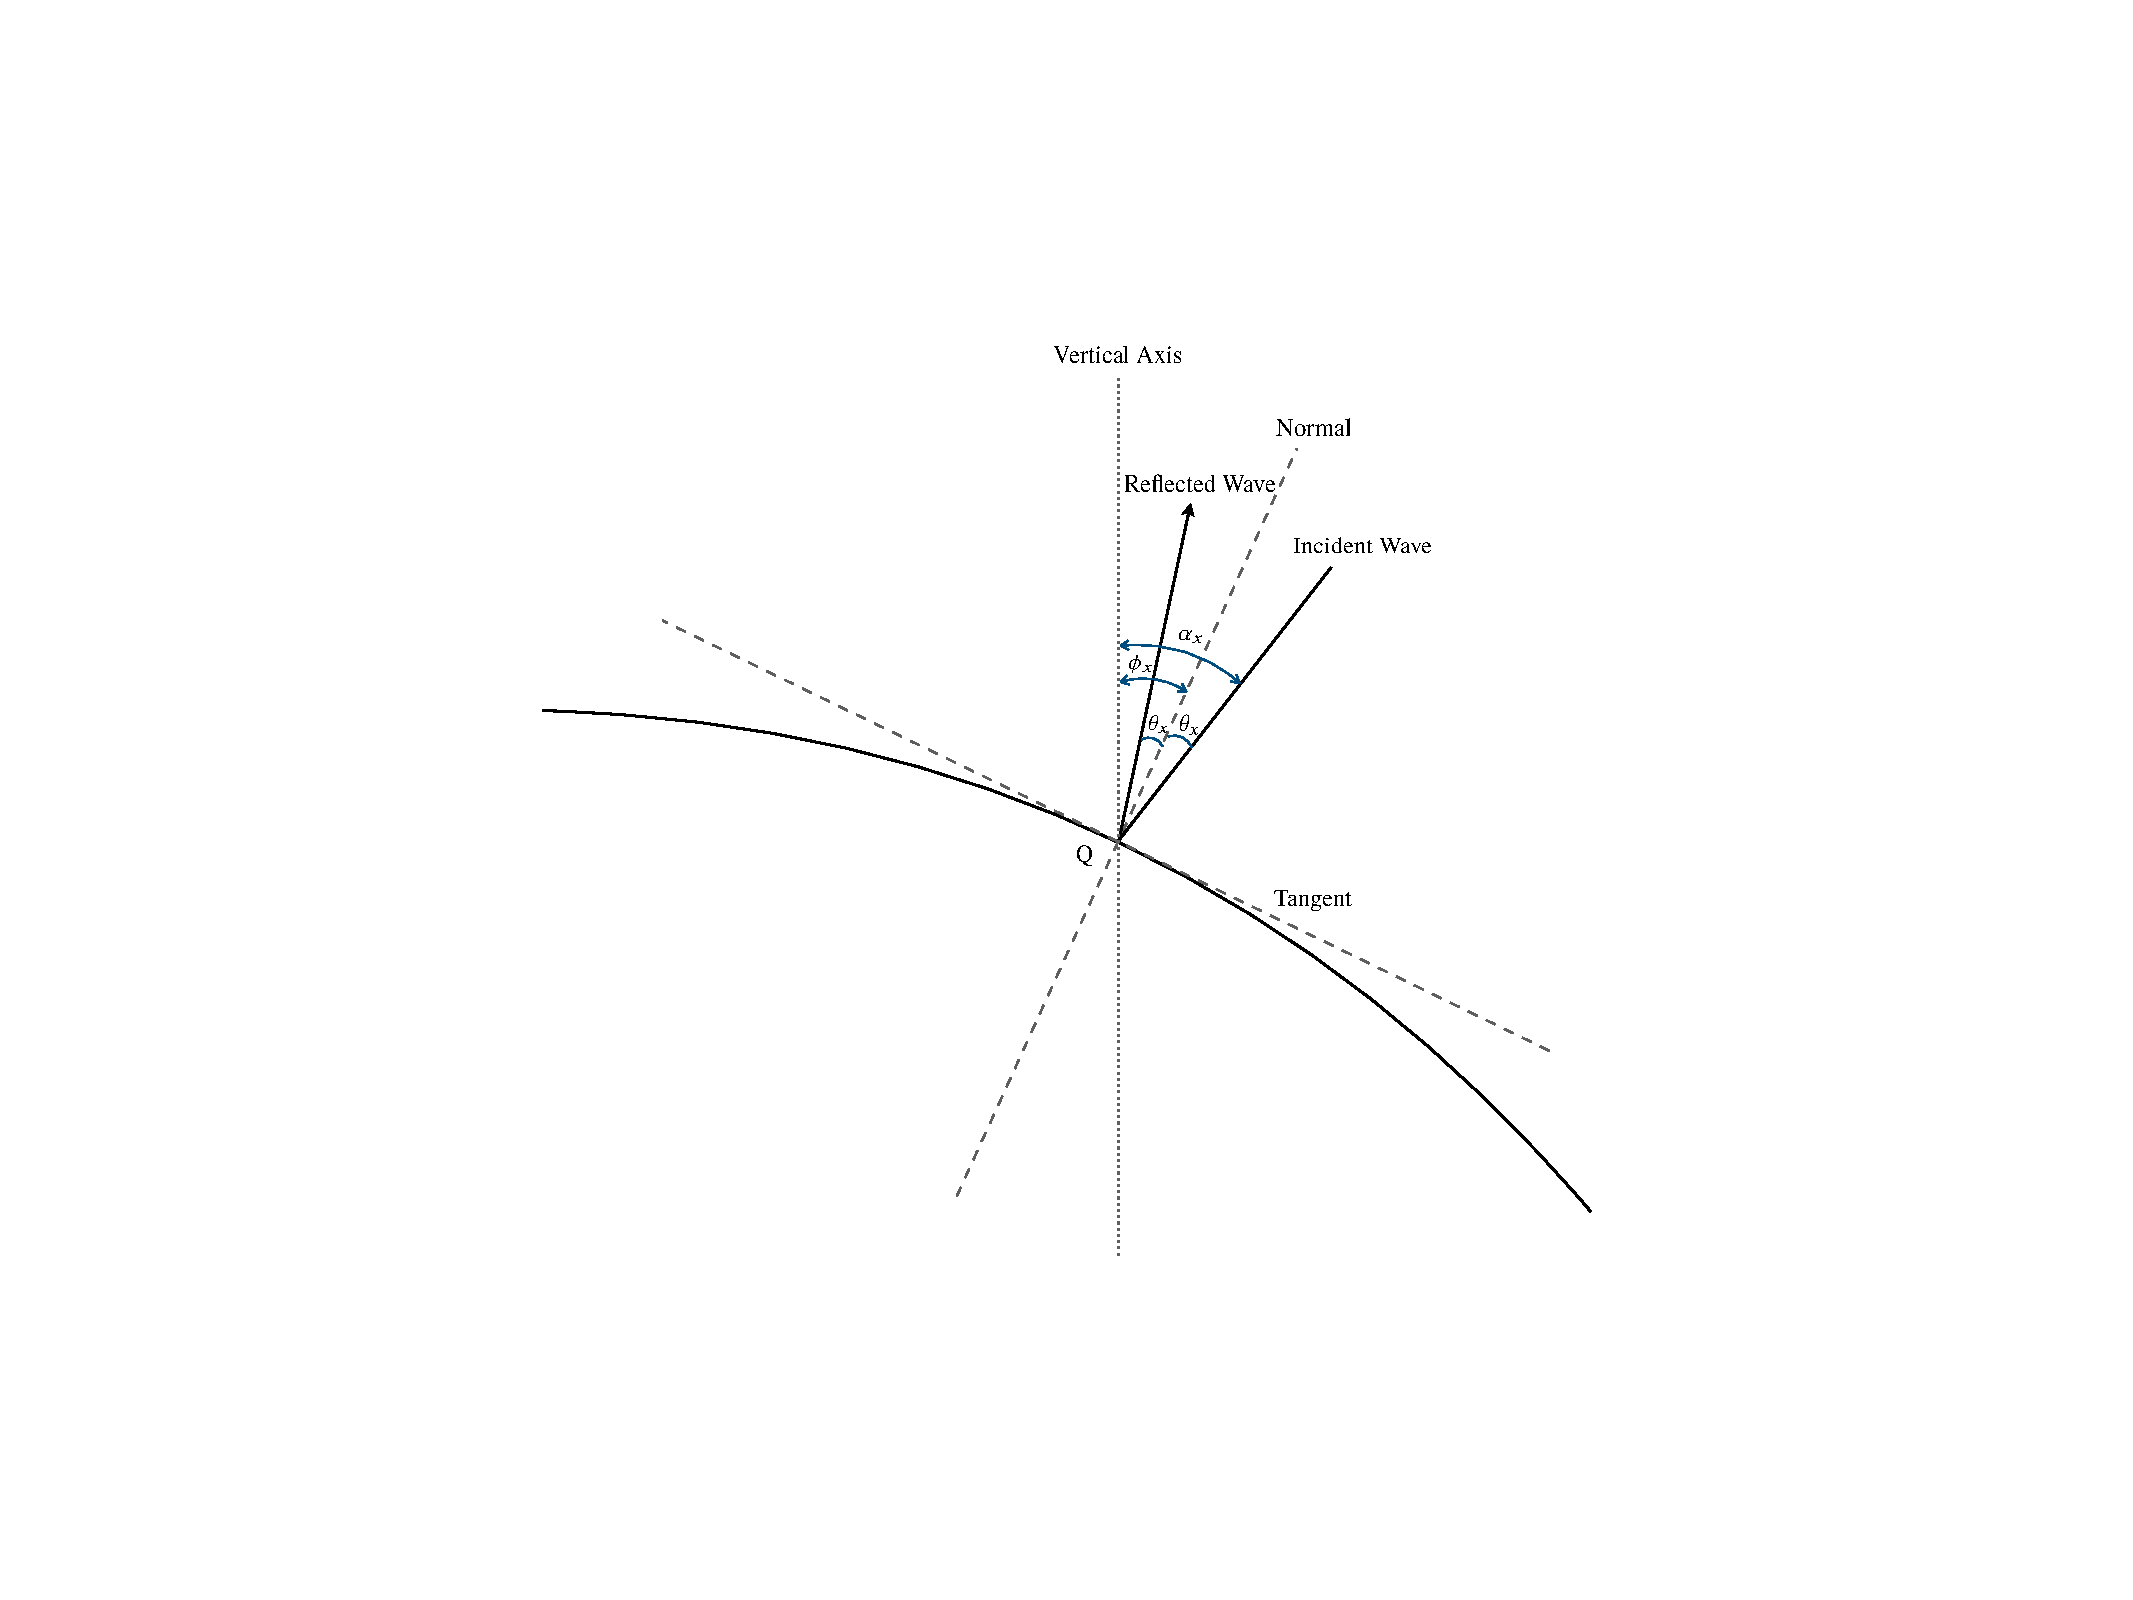
\includegraphics[width=420,height=310,clip,trim=200 150 200 150]{angle-rel.pdf}
    \caption{Relationship between angle $\alpha$, $\theta$ and $\phi$ for $x$-$z$ and $x$-$y$.}
    \label{fig:angle_rel}
\end{figure}

The total angle of deviation of each angle from the vertical axis can also be expressed in terms of their $x$ and $y$ components.

\begin{equation}\label{eqn:alpha_rel}
    \alpha = \arctan\left(\sqrt{\tan^2\alpha_x + \tan^2\alpha_y}\right)
\end{equation}
\begin{equation}\label{eqn:theta_rel}
    \theta = \arctan\left(\sqrt{\tan^2\theta_x + \tan^2\theta_y}\right)
\end{equation}
\begin{equation}
    \phi = \arctan\left(\sqrt{\tan^2\phi_x + \tan^2\phi_y}\right)
\end{equation}

We utilize equation \eqref{eqn:prob} to obtain
\begin{equation}
    P(\theta_x,\theta_y, \alpha_x, \alpha_y) = \frac{1}{2\pi \sigma_x \sigma_y \sqrt{1 - \rho^2}} \exp\left[-\frac{1}{2(1-\rho^2)}\left(\frac{(\theta_x - \alpha_x)^2}{\sigma_x^2} + \frac{2\rho (\theta_x - \alpha_x) (\theta_y - \alpha_y)}{\sigma_x \sigma_y} + \frac{(\theta_y - \alpha_y)^2}{\sigma_y^2}\right)\right]
\end{equation}

This is a probability density function for the relative angle of incidence, when $\alpha_x$ and $\alpha_y$ are given. By using equation \eqref{eqn:r_total}, we can find the expected reflectance for an electromagnetic wave incident on a turbulent ocean with roughness $\sigma_x$ in the $x$-axis and $\sigma_y$ in the $y$-axis:
\begin{equation}
    R\left(\sigma_x,\sigma_y,\alpha_x,\alpha_y\right) = \int_{-\frac{\pi}{2}}^\frac{\pi}{2} \int_{-\frac{\pi}{2}}^\frac{\pi}{2} r\left[\arctan\left(\sqrt{\tan^2\theta_x + \tan^2\theta_y}\right)\right] P\left(\theta_x, \theta_y, \alpha_x, \alpha_y \right) d\theta_x d\theta_y
\end{equation}

Due to the complexity of the equation above, we are unable to compare it with the reflectance of radio waves on calm ocean surface.

\subsubsection{Signal Strength in the Atmosphere} 

After the radio wave signal is incident on the water surface, it travels back to the atmosphere into the ionosphere (50 - 600 km). The ionosphere is often divided into distinct layers, each with different properties regarding their ionization level. The lowest level is known as the D level, ranging from 50-90 km in altitude. It has an attenuating effect mainly on electromagnetic waves of low frequency, and it disappears at night.

Unlike the D layer, the E and F layer of the ionosphere have lower air densities and higher electron density. When an electromagnetic signal enter these layers, they cause electrons to vibrate at the same frequency as the signal itself (if the frequency is below the maximum usable frequency), and they re-radiate the signal back to the ground at the same angle as the angle of incidence. In order for a wave to be reflected by either layer, it must cross the D layer twice, where it is attenuated. The first part of the model will focus on calculating the proportion of strength lost by a radio wave of a specific frequency when it is reflected from the ionosphere. Although the ionosphere is complicated and varies from time to time in terms of its structure, we simplify its properties by using continuous probability distributions.

The attenuating effect of the D-layer of the ionosphere is due to the presence of air molecules that collide with vibrating electrons that are excited by electromagnetic signals that pass through the layer. It is known that the attenuation effect of a signal is proportional to the pressure of air that it travels. NASA has provided a model for the relationship between pressure ($p$ in \emph{lbs/sqft}) and altitude ($h$ in \emph{ft}), as shown in equation \eqref{eqn:pressure_altitude}.

\begin{equation}\label{eqn:pressure_altitude}
p(h) =\begin{cases}
51.97\left(\frac{459.7\, +0.00164 h-205.05}{389.98}\right)^{-11.388} & h>82345 \\[14pt]
 473.1 e^{1.73\, -0.0000483 h} & 36152\leq h\leq 82345 \\[12pt]
 2116 \left(\frac{459.7\, -0.00356 h+59}{518.6}\right)^{5.256} & 0\leq h<36152
\end{cases}
\end{equation}

After a quick conversion from the British metric system to SI units, we can express pressure in atmospheres (atm) in terms of altitude $h$ in meters.

\begin{figure}[htbp]
    \centering
    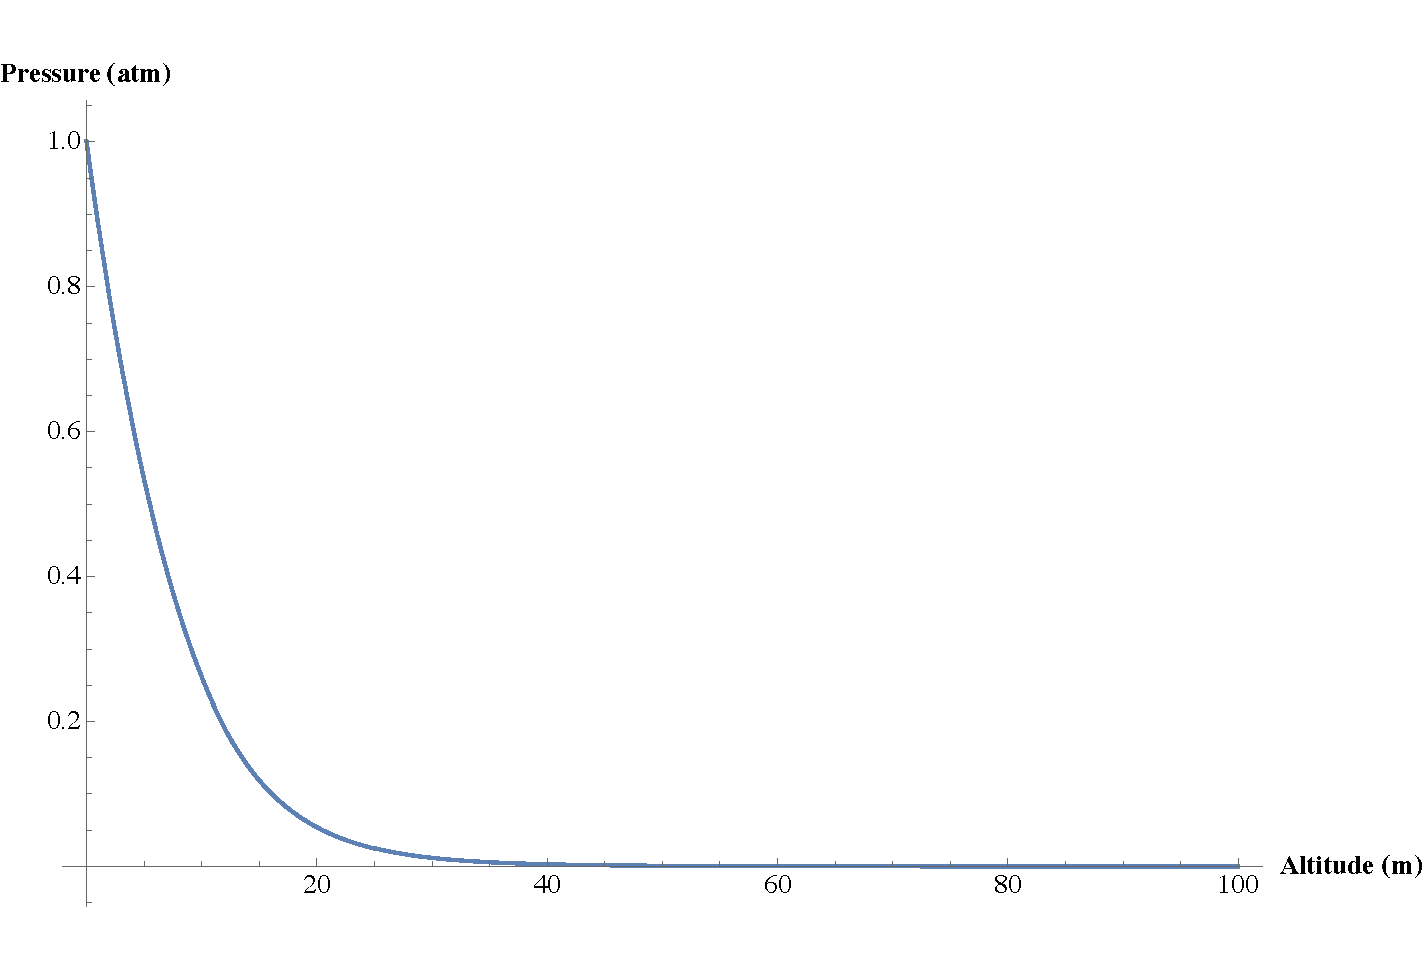
\includegraphics[scale=.6,clip,trim=0 30 0 15]{pressure_plot_2d.pdf}
    \caption{Relationship of pressure and altitude.}
    \label{fig:pressure_plot_2d}
\end{figure}

Let $c$ be the \textbf{constant of proportionality} that relates the pressure of air and the strength that is absorbed in the D-layer. This can be achieved by computing a line integral alone the direction of the wave. First consider a scalar field $S = cp(h)$ that represents the attenuation intensity of the D-layer at each point. To simplify the model, we will assume that the region which the wave propagates in the atmosphere is flat, and that the distribution of free electrons and air pressure are uniform across all points within the same altitude. Let the angle of elevation $\psi$ to be given, and let the $x$-$z$ plane to contain the straight path $L$ of the path of the incident radio wave.

The total strength that is lost while the wave propagates through a region of varying To compute the line integral along $L$, we must find a parameterization that traces $L$. We set the $x$-$z$ coordinate system such that $\gamma(0)$ is at $(0,0)$ and $\gamma(1)$ = $\left(\frac{40000}{\tan \psi},40000\right)$:

\begin{equation}
L \text{ parameterization}:\begin{cases}
x = \frac{t}{\tan \psi} \\[10pt]
z = 50000+t
\end{cases}, 0 \le t \le 40000.
\end{equation}

This implies that $\displaystyle\frac{dx}{dt} = \cot\psi$ and $\displaystyle\frac{dz}{dt} = 1.$

The line integral of $cp(h)$ along $L$ can be expressed as the attenuation $A(\psi)$ that expresses the strength of the attenuation depending on the angle of elevation of the incoming signal: 
\begin{align}
    A \left(\psi\right) & = \int_L cp\left(h\right) ds\\
    & = c \int_0^{40000}p\left(50000 + t\right) \sqrt{\left(\frac{dx}{dt}\right)^2 + \left(\frac{dz}{dt}\right)^2}dt \\
    & = c \int_0^{40000} p\left(50000 + t\right) \sqrt{\cot^2 \psi + 1} dt \\
    & = c\, 5.49071\times 10^{-31} \csc(\phi).
\end{align}

Apparently, $c$ needs to be a considerably large number in order for the path $L$ to have a noticeable effect in attenuating the radio wave. This is reasonable because the pressure at around 50 km above sea level is tiny comparing to the atmospheric pressure at the surface of the ocean.

\begin{figure}[htbp]
    \centering
    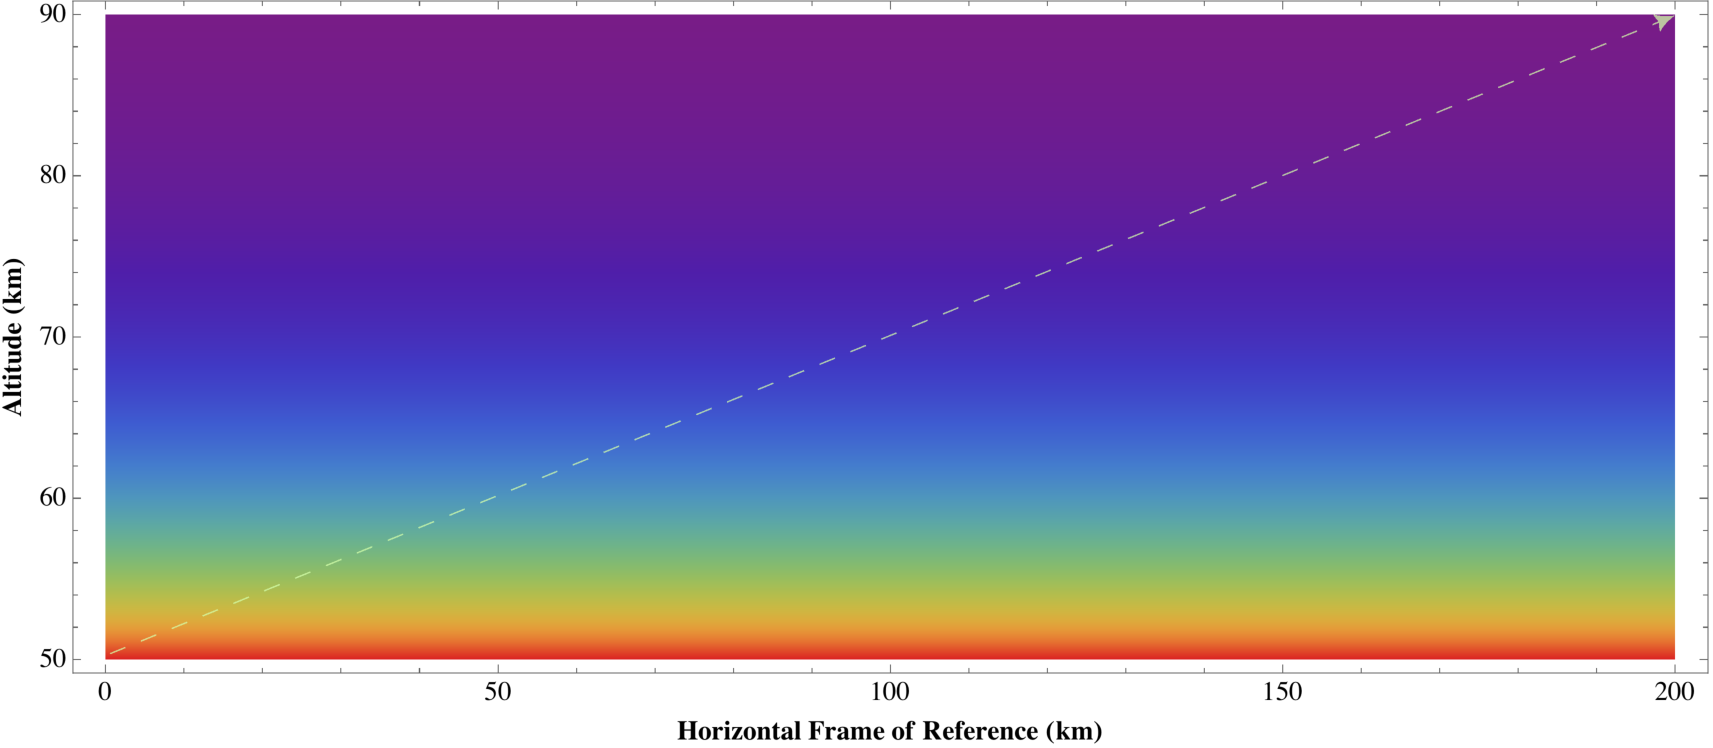
\includegraphics[scale=.51]{pressure_density_plot.pdf}
    \caption{Visualization of path crossing air of varying density.}
    \label{fig:pressure_density_plot}
\end{figure}

It is also known that the attenuation effect varies with the frequency of the radio signal. More specifically, the attentuation effect $A(\psi)$ varies proportionally with the inverse square of the frequency $f$. This means that
\begin{equation}
    A(\psi) = kf
\end{equation}
where $k$ is an unknown constant of proportionality. 

% The frequency of the emitted wave is \emph{HF}, meaning that it ranges between 3-30 MHz. 

\subsubsection{Angle and Direction of Reflection}
For any given spatial line in vector form $\vec{r}=\vec{a}+\lambda\vec{u}$ and any spacial surface $y=f(a_1,\cdots,a_n)$, the intersection thereof would be $\vec{r}(\lambda)$ where $\lambda$ is the solution of
\[
\left|\vec{r}(\lambda)\cdot\hat{i}_{n+1}\right|=f\left(\left|\vec{r}(\lambda)\cdot\hat{i}_{1}\right|,\cdots,\left|\vec{r}(\lambda)\cdot\hat{i}_{n}\right|\right)
\]

Tangent hyper-plane equation of function $y=f(x_1,\cdots,x_n)$ at intersection point $\displaystyle{P\left(a_1,\cdots,a_n,f\left(x_1,\cdots,x_n\right)\right)}$ is
\begin{gather}
\label{eqn:tangent_eqn_multi}
y=\sum_{i=1}^n\frac{\partial f}{\partial x_i}(a_1,\cdots,a_n)\cdot x_i-\sum_{i=1}^n\frac{\partial f}{\partial x_i}(a_1,\cdots,a_n)\cdot a_i+f(x_1,\cdots,x_n)
\end{gather}

The normal vector of the hyper-plane above would be deducted from (\ref{eqn:tangent_eqn_multi}),
\begin{gather}
\label{eqn:normal_at_point}
\vec{N}=\left<\frac{\partial f}{\partial x_1},\cdots,\frac{\partial f}{\partial x_n},-1\right>
\end{gather}
and the alternative method for evaluating this is to employ the \textbf{Hodge Dual} of their tensor product and multiply it by $(n-1)!$.

Without loss of generality, we assume that $\vec{N}+P\geq f\left(x_1,\dots,x_n\right)$, and if otherwise then the opposite vector of $\vec{N}$, namely $-\vec{N}$ can be taken as replacement thereof.

Now denote the vector indicating the direction of the incoming light as $\vec{p}=\vec{u}$, and the outcoming light, $\vec{q}$, and the normal plane in which reflection phenomenon takes place will be solved by the standard Normal-Point form of the plane and cross product.

Since the angle between $\vec{N}$ and $\vec{q}$, $\theta$, can be defined as $\theta=\pi-\theta$, where $\gamma$ is the angle between $\vec{N}$ and $\vec{p}$
\begin{gather}
\label{eqn:cosrule}
\frac{\vec{p}\cdot\vec{N}}{\left|\vec{p}\right|\cdot\left|\vec{N}\right|}=\cos\gamma=\cos(\pi-\theta)=-\cos\theta=-\frac{\vec{q}\cdot\vec{N}}{\left|\vec{q}\right|\cdot\left|\vec{N}\right|}
\end{gather}

With the above (\ref{eqn:cosrule}), along with the fact that the normal vector of the normal is normal to $\vec{q}$, in another word they are co-linear, which means $\vec{q}\cdot\left(\vec{p}\times\vec{N}\right)=0$, we are now able to solve $\vec{q}$ in $n$-dimensional Euclidean spaces.

The specialized form of (\ref{eqn:tangent_eqn_multi}) for bi-variate functions is
\begin{gather}
\label{eqn:tangent_eqn_bivar}
z=\frac{\partial f}{\partial x\cdot}(x_0,y_0)\cdot x+\frac{\partial f}{\partial y}(x_0,y_0)\cdot y-\frac{\partial f}{\partial x}(x_0,y_0)\cdot x_0-\frac{\partial f}{\partial y}(x_0,y_0)\cdot y_0+f(x_0,y_0)
\end{gather}

The specialized procedure written in Mathematica determining the outcoming reflection ray is augmented in the Appendix \ref{apdx:omega_3}
\subsubsection{Attenuation of Wave in the Atmosphere}
\begin{itemize}
    \item \textbf{Absorption of Radio Wave by Vapor}
    
    \begin{gather}
    \label{eqn:a_vapor}
    A_v = 
    \begin{cases}
    \displaystyle\frac{h_v\lambda_v}{\sin(El)}\\[14pt]
    \displaystyle\lambda_v\frac{\sqrt{R_e \cdot h_v}}{\cos(El)}\cdot F(\tan(El)\cdot \sqrt{\frac{R_e}{h_v}})
    \end{cases}
    \end{gather}
    $El$ is the angle of elevation, $R_e$ is the effective radius of Earth.
    
    \item \textbf{Absorption of Radio Wave by Oxygen}
    
    \begin{gather}
    \label{eqn:a_cloud}
    A_v = 
    \begin{cases}
    \displaystyle\frac{h_o\lambda_o}{\sin{El}}\\[12pt]
    \displaystyle\lambda_v\frac{\sqrt{R_e \cdot h_o}}{\cos{El}}\cdot F(\tan{El}\cdot \sqrt{\frac{R_e}{h_v}})
    \end{cases}
    \end{gather}
    
    \item \textbf{Attenuation of Radio Wave by Raining}
    
    
    
    \item \textbf{Attenuation of Radio Wave by Cloud}
    
    \begin{gather}
    \label{eqn:a_cloud}
    A_c = \displaystyle\frac{\Delta h \cdot \lambda_c}{\sin{El}}
    \end{gather}
    
    \item \textbf{Attenuation of Radio Wave by Ionosphere}
\end{itemize}
\subsection{Part II}
\subsection{Part III}
\section{Result}
\section{Conclusion}
\section{Strengths and Weaknesses}
\subsection{Strength}
\begin{itemize}
    \item We tried.
\end{itemize}
\subsection{Weakness}
\begin{itemize}
    \item Due to the existence of ionospheric disturbance, the electromagnet wave emitted to the ionosphere would be heavily impacted and attenuated. Such influence are significant and unpredictable. 
    \item We are unable to finish this essay because of the lack of essential knowledge in physics. We will participate in this contest again when we go to college.
\end{itemize}
\section{Appendices}
\subsection{Calculation of Reflective Index of Average Ocean Surface} \label{}

\subsection{Standard Deviation of Ocean Surface Turbulence} \label{sd}
We used the ocean surface data from NASA (file:'ssh\_grids\_v1609\_2017123012\_i.nc'). We measured slopes between every two points and calculated the standard deviation using Matlab.
\newpage

\appendix
\section{Reflection 3D $\omega_3$}
\label{apdx:omega_3}
%%%%%%%%%%%%%%%%%%%%%%%%%%%%%%%%%%%%%%%%%%%%%%%%%%%%%%%%%%%%%%%%%%%%%%%%%%%%%
\begin{mmaCell}[morepattern = {f_,  a_,  u_,  a,  u,  f,  \#,  \#1,  \#2}, morelocal = {P,  r,  n,  p,  s,  q}, moredefined = {VectorAngle}]{Input}
  \mmaDef{\(\pmb{\omega}\)3}[f_, a_, u_]: = Module[\{\mmaLoc{\(\pmb{\lambda}\)0}, P, r, n, p, s, q = \{q1, q2, q3\}, \mmaLoc{\(\pmb{\theta}\)1}, \mmaLoc{\(\pmb{\theta}\)2}\}, 
    r = a + \mmaUnd{\(\pmb{\lambda}\)} u;
    \mmaLoc{\(\pmb{\lambda}\)0} = \mmaUnd{\(\pmb{\lambda}\)} /. Solve[r[[3]] == f[r[[1]], r[[2]]], \{\mmaFnc{\(\pmb{\lambda}\)}\}];
    P = r /. \mmaUnd{\(\pmb{\lambda}\)} \(\pmb{\to}\) First@Sort@Select[\mmaLoc{\(\pmb{\lambda}\)0}, # \(\pmb{\geq}\) 0&];
    p = P - a;
    n = \{
        D[f[x, y] /. <|x \(\pmb{\to}\) P[[1]], y \(\pmb{\to}\) P[[2]]|>, x], 
        D[f[x, y], y] /. <|x \(\pmb{\to}\) P[[1]], y \(\pmb{\to}\) P[[2]]|>, 
        -1
    \};
    If[n + P < f@@P, n = -n];
    s = n \(\pmb{\times}\) p;
    \mmaLoc{\(\pmb{\theta}\)1} = VectorAngle[-p, n];
    \mmaLoc{\(\pmb{\theta}\)2} = VectorAngle[q, n];
    q = \{q1, q2, q3\} /.
        Solve[\{
            Norm[q] == Norm[p], 
            q . s == 0, 
            \mmaLoc{\(\pmb{\theta}\)1} == \mmaLoc{\(\pmb{\theta}\)2}
        \}, \{\mmaFnc{q1}, \mmaFnc{q2}, \mmaFnc{q3}\}];
    If[\mmaLoc{\(\pmb{\theta}\)1} == 0, Return[-p]];
    If[\mmaLoc{\(\pmb{\theta}\)1} == \mmaDef{\(\pmb{\pi}\)}, Return[p]];
    First@First@Sort[\{#, Min[VectorAngle[p, #], VectorAngle[-p, #]]\}& /@ q,
        #1[[2]] > #2[[2]]&]
  ];
\end{mmaCell}
%%%%%%%%%%%%%%%%%%%%%%%%%%%%%%%%%%%%%%%%%%%%%%%%%%%%%%%%%%%%%%%%%%%%%%%%%%%%%

\newpage
\begin{thebibliography}{9}
\bibitem{Surface}
W. I. Roderick and R. L. Deavenport, “Doppler characteristics of sea surface reflected and scattered acoustic signals induced by surface wave motion,” in OCEANS 1993, Victoria, BC, Canada (1993), pp. I287–I292.

\bibitem{a}
Zhao, Xiaofeng, and Sixun Huang. \textit{Influence of Sea Surface Roughness on the Electromagnetic Wave Propagation in the Duct Environment.} Institute of Meteorology, PLA Univ. of Sci. & Tech., Nanjing 211101, China , pdfs.semanticscholar.org/2d10/4939ea92272cb527e732d4ac5f7dd310a30d.pdf.

\bibitem{b}
Takashi, Ichiye. \textit{Reflection of electromagnetic waves at sea surface.} Société franco-Japonaise d'Océanographie, www.sfjo-lamer.org/la\_mer/28-2\_3/28-2-3-1.pdf.

\bibitem{c}
“Fresnel's Equations.” \textit{Fresnell's Equations: Reflection and Transmission}, hyperphysics.phy-astr.gsu.edu/hbase/phyopt/freseq.html. 


\bibitem{d}
“Fresnel equations.” Wikipedia, Wikimedia Foundation, 11 Feb. 2018, en.wikipedia.org/wiki/Fresnel\_equations. 

\bibitem{e}
Jones, Edwin C. “The Basics of Radio Wave Propagation.” \textit{Basics of Radio Wave Propagation}, ecjones.org/propag.html

\bibitem{f}
“Ionospheric Radio Wave Propagation.” \textit{National Oceanic and Atmospheric Administration}, www.ngdc.noaa.gov/stp/space-weather/online-publications/miscellaneous/afrl\_publications/handbook\_1985/Chptr10.pdf.

\bibitem{g}
“Modeling the variations of reflection coefficient of Earth's lower ionosphere using very low frequency radio wave data by artificial neural network.” \textit{Advances in Space Research}, Pergamon, 9 May 2016, www.sciencedirect.com/science/article/pii/S0273117716301624.

\bibitem{h}
Jones, Edwin C. “Ionospheric Physics of Radio Wave Propagation.” \textit{Ionospheric Physics of Radio Wave Propagation}, ecjones.org/physics.html.

\bibitem{i}
Radio Waves Propagation. \textit{IDC technologies}, www.idc-online.com/technical\_references/pdfs/electronic \_engineering/Radio\_Waves\_Propagation.pdf.

\bibitem{j}
“D Layer Absorption.” \textit{Ham Radio School.Com}, 13 Oct. 2015, www.hamradioschool.com/d-layer-absorption/.

\bibitem{k}
“What is the scale height of water vapour in the Earth's atmosphere?” \textit{Thecuriousastronomer}, 27 June 2016, thecuriousastronomer.wordpress.com/2016/06/27/what-is-the-scale-height-of-water-vapour-in-the-earths-atmosphere/. 

\bibitem{l}
Klima, Ján, and Marián Možucha. \textit{Influence of Terrain on Multipath Propagation of FM Signal}. Slovenská Technická Univerzita V Bratislave, iris.elf.stuba.sk/JEEEC/data/pdf/05-06\_105-01.pdf.

\end{thebibliography}

\end{document}